One of the mains features of this work is to have shown that, independently of its condition, the microbiota follows the Taylor's law. We have seen that the value of the scaling index in each case is always less than the unity (using standard deviation as the measurement for dispersion), which is informing us about the community structure. This means that, in relative terms, the most abundant elements in the population are less volatile to perturbations than the less abundant ones. The explanation for this universal pattern is not clear although some hypothesis have been tested in other studies, as the presence of negative interactions in the population \cite{kilpatrick}, or the demonstration that it may depend on reproductive correlation \cite{ballantyne}. Nevertheless, none of these explanations are enough when we are talking about microbiota as the reproduction term is diffuse, the interactions between its components are not only based on competition \cite{joao, mehta, bucci} and that even that kind of negative interaction may not effectively yield in values less than the unity when referring to a bacterial species \cite{ramslayer}. Anyhow, the values obtained in all cases are very similar among them, which could be suggesting that the community structure is preserved throughout the different scenarios that we have studied.

The second parameter is informing about the noise and can be directly related with the variability or the fluctuation amplitude of the population over time. It is a direct estimator of the stability of the system under study. As we showed above, the healthy subset of each study have lower variability than the non-healthy subset when dealing with adult individuals. Interestingly, the variability parameter was higher in the healthy subset for the study of the discordant twins suffering from kwashiorkor disease \cite{kwashiorkor}. In this regard it has been shown that the infant microbiota needs to develop toward a definite, adult state \cite{koenig}. This implies that the temporal variability would be greater in children respect to a healthy adult state, which should be temporally stable. Thus, our results could be pointing out the need of this variability in order to reach that adult state. Furthermore, as we wanted to see how this variability behaved over time, we calculated the evolution of this parameter for the samples which had enough time sampling. As can be seen in Figure \ref{fig:tempevo1}, the variability of the microbiota has some fluctuations over time. It is interesting to note in Figure \ref{fig:tempevo2} how this parameter can capture the two antibiotic intakes in one of the patients from the study of Dethlefsen and Relman \cite{antibiotic}, especially that it seems to be some resilience process in the microbiota due to the lower variability increase in the second antibiotic intake.  

The primary hypothesis of this work is that, in adults, having a healthy microbiota means that population is stable in time and does not travel into a state where it is highly susceptible to external or internal perturbations, causing in such a case a dysbiotic state in the microbiota. In order to use the valuable information which gives us the empirical law of Taylor's work, we propose the use of Langevin equation to model how the ranking stability evolves in time. While we can measure directly the component of the noise of the system as their variability, the other main term needs to be inferred from the model. This term, which we have named as 'fitness', is the one that gives the ability to the system to be stable to potential perturbations. In ecological terms, this could mean the nature of interactions that are present among the bacteria, between bacteria and other minority populations as fungi or archaea, between bacteria and the viral component in the microbiota, and the interactions between host and the whole microbiota. Being this a first step to model the temporal stability of the microbiota and due to its complicated nature, we have calculated the fitness term using the Fluctuation Dissipation Theorem as a first approximation\cite{FD}. Thus, the fitness of the microbiota still remains to be modelled in future works in order to make the model more accurate and with a higher predictive power. 

By solving the Langevin differential equation, we can obtain a phase diagram where each microbiota sample can be placed according to its fitness and variability in one of two phases according to the ranking stability of the system. As we can see in the phase-space in Figure \ref{fig:main3}, we are showing three different conditions that could happen. First, we can have a healthy microbiota which could have some fluctuations as showed by one of the subjects of Caporasso et al study \cite{moving}. Because the fitness of this cases will be high enough, the temporal variability will not place the microbiota in the unstable phase of the diagram. Second, we have a subject from the study of Dethlefsen and Relman \cite{antibiotic} which is perturbed twice by an antibiotic intake. His microbiota is altered enough to lose its stability, and hence be placed in the unstable part. So located, it is more sensitive to potential perturbations as, for example, opportunist infections. Third and last condition, the subject is already in the unstable phase due to some healthy issue as IBS. This can be observed in one of the patients from Durban et al study \cite{IBS}. In addition, it was shown that this subject improved its healthy status in the time when the experiment was done, implying that his microbiota also recovered the lost stability. It is interesting to notice that in the subject from the study of David et al. \cite{hostlife}, who suffered a Salmonella infection during the experiment, we can observe a huge shift in the variability and a final recovery from the perturbed state (see \ref{supfig:HLS_xWSummary}).

\begin{supfig}
	\centering
	%\vspace*{-10mm} % Corrects overbox of the figures
	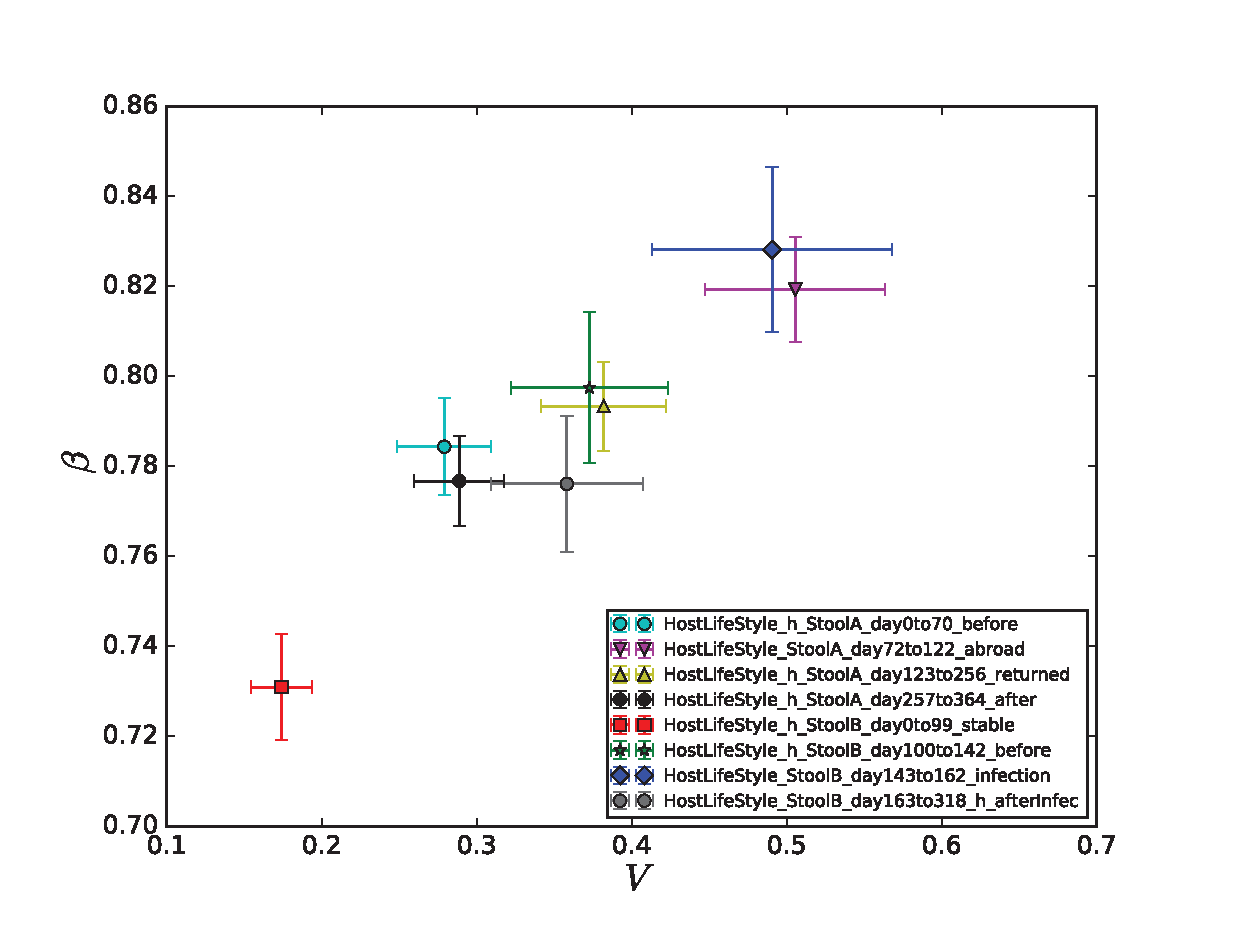
\includegraphics[width=0.99\textwidth]{figs/supfig_HLS_xWSummary.eps}
	\caption{Taylor's law parameter space for intervals concerning gut microbiota in the host lifestyle study\cite{hostlife}.}
	\label{supfig:HLS_xWSummary}
\end{supfig}
 
Specifically, the analysis of the rank stability of the samples of healthy and IBS diagnosed patients studied in our lab\cite{IBS}, suggests that the presence of \emph{rank stability islands} among medium-ranked taxa is a interesting feature. The higher stability of these taxa goes against the global meaning of the scaling index. Interestingly, that stability disappears when we look at the IBS patients. From the literature, it seems that some genera from the families Comamonadaceae, Neisseriaceae and Carnobacteriaceae have been reported to lower their abundance in IBS patients against healthy controls \cite{sislands1}. In our case, we see that these families that are present in the rank stability island of the healthy patient decrease their rank stability index or even disappear in the IBS patient. However, we also see contradictory results in other families as Lactobacillaceae or Fusobacteriaceae, which seems to increase their abundance in IBS patients \cite{sislands2}, while we observe an increase of the former and a decrease of the latter. The presence of members of the Lactobacillae family have been reported to have positive effects against gut inflammation and visceral hyperalgesia \cite{sislands3}, usual symptoms of gastrointestinal disorders. It could be happening that a disorder in the stability of this particular group may help to arise the onset of symptoms associated to gastrointestinal disorders. The Aerococacceae family is also enriched in rats with IBS symptoms who have been treated with immunomodulators \cite{sislands4}. Inside this island of stability, we also have families as Fusobacteriaceae o Hallomonadaceae which include pathogenic genera in them, but that are not present in the IBS patient. It could be brought into question the rule of these taxa as key players in the phase transition of the microbiota, or whether they are more susceptible to perturbations than the most abundant. The types of interactions that could be sustaining this particular behavior are not clear, as these non-abundant taxa are not usually included in dynamical studies in order to get the community matrix. Further experiments and data analysis is needed to clarify if this is not a unique event, or it is a widespread feature of stable microbiotas. 

However, we have to be aware that the hypothesis above is too simplistic to be directly related with reality. It has been demonstrated that the situation is more complex than the outlook provided separating healthy people from non-healthy people just by compositional terms, as Moya and Ferrer underline in their recent review \cite{Moya_trends}. There are several different feasible scenarios in which we can consider the microbiota as stable independently of their compositional evolution over time. For example, depending on their ability to recover the initial composition (resilience), or whether it can recover the original function despite the composition (functional redundancy). What we have shown in this work could be explained as the transitions of a stable microbiota into a dysbiosis state.  

As a first step toward understanding the microbiota stability, the model presents some limitations and there is still work to do. From the biological perspective, many questions arise from this work. We have observed the same pattern in Taylor's parameters in all the different conditions we have studied, but a pertinent question is whether it is really a universal feature in the huge diversity of microbial niches. Furthermore, another relevant question is which mechanisms are involved in maintaining the population structure. The nature of the interactions among the elements of the community is surely of great importance in this matter, and it is related to the fitness of the community as has been commented above. How we should address the community fitness is not clear, but works as Tikhonov's \cite{tikhonov} could help us to aim at the correct direction toward unraveling the complexity of the microbiota.